\documentclass[12pt,a4paper]{article}
\usepackage[utf8]{inputenc}
\usepackage[spanish]{babel}
\usepackage{amsmath}
\usepackage{amsfonts}
\usepackage{amssymb}
\usepackage{graphicx}
\usepackage{kpfonts}
\usepackage[left=2cm,right=2cm,top=2cm,bottom=2cm]{geometry}
\title{EV 1-2 OPTOACOPLADORES Y RELEVADORES

\includegraphics [scale=1]{imagenes/UPZMG.png} 
\author{Giovanni Daniel Ruiz Tinoco\\
Alan Antonio Muñoz Juarez\\
\small Sistemas electrónicos de interfaz\\
  \small Universidad Politécnica de la zona metropolitana de Guadalajara\\
  \small 4-B \\
  \small Ing. Mecatrónica\\
\centering
}
}
\begin{document}
\maketitle
\newpage
\begin{center}
\section {MARCO TEÓRICO}
\subsection{Optoacopladores}
\end{center}
Un optoacoplador, también llamado optoaislador o aislador acoplado ópticamente, es un dispositivo de emisión y recepción que funciona como un interruptor activado mediante la luz emitida por un diodo led que satura un componente optoelectrónico, normalmente en forma de fototransistor o fototriac. De este modo se combinan en un solo dispositivo semiconductor, un fotoemisor y un fotorreceptor cuya conexión entre ambos es óptica. Estos elementos se encuentran dentro de un encapsulado que por lo general es del tipo DIP. Se suelen utilizar para aislar eléctricamente a dispositivos muy sensibles.\linebreak

Además de para aislar circuitos, se pueden utilizar optoacopladores para:\\
-Interfaces en circuitos lógicos.\\
-Interfaces entre señales de corriente alterna y circuitos lógicos.\\
-En sistemas de recepción (telefonía).\\
-Control de potencia.\\
-A modo de relé.\\
\begin{center}
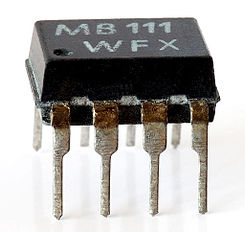
\includegraphics[scale=1]{imagenes/opto.jpg}  
\newpage
\subsection{Relevadores}
\end{center}
\begin{flushleft}
Un relevador es un aparato eléctrico que funciona como un interruptor pero que es accionado eléctricamente. El relé permite abrir o cerrar contactos mediante un electroimán, Fue desarrollado en la primera mitad del siglo XIX por el físico norteamericano Joseph Henry, a través de una bobina y un electroimán.
Lo que hace la bobina es crear un campo magnético que lleva los contactos a establecer una conexión. El electroimán, por su parte, permite el cierre de los contactos
\end{flushleft}
\begin{center}
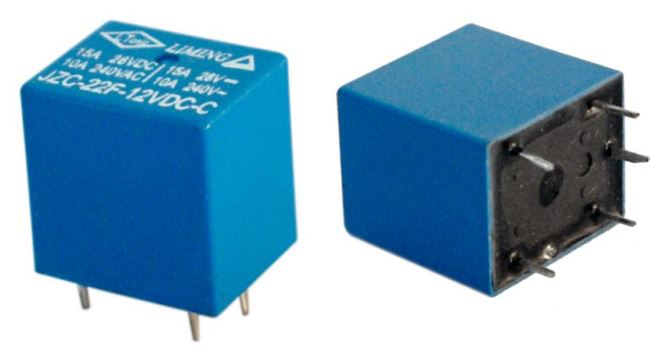
\includegraphics[scale=1]{imagenes/rele.JPG} 
\end{center}
Un relevador funciona como un interruptor controlado por un circuito eléctrico en el que, por medio de una bobina y un electroimán, se acciona un juego de uno o varios contactos que permiten abrir o cerrar otros circuitos eléctricos independientes.
Dado que el relé es capaz de controlar un circuito de salida de mayor potencia que el de entrada, puede considerarse, en un amplio sentido, como un amplificador eléctrico.\\
\newpage
\begin{center}
\subsection{Materiales para la práctica}
\end{center}
\begin{flushleft}
-3 Optoacopladores\\
-3 Relevadores (12v o 5v)\\
-3 Led \\
-Resistencias variadas\\
-Arduino \\
-Protoboard\linebreak

Realice la simulación y el circuito del siguiente esquema:\\
\end{flushleft}
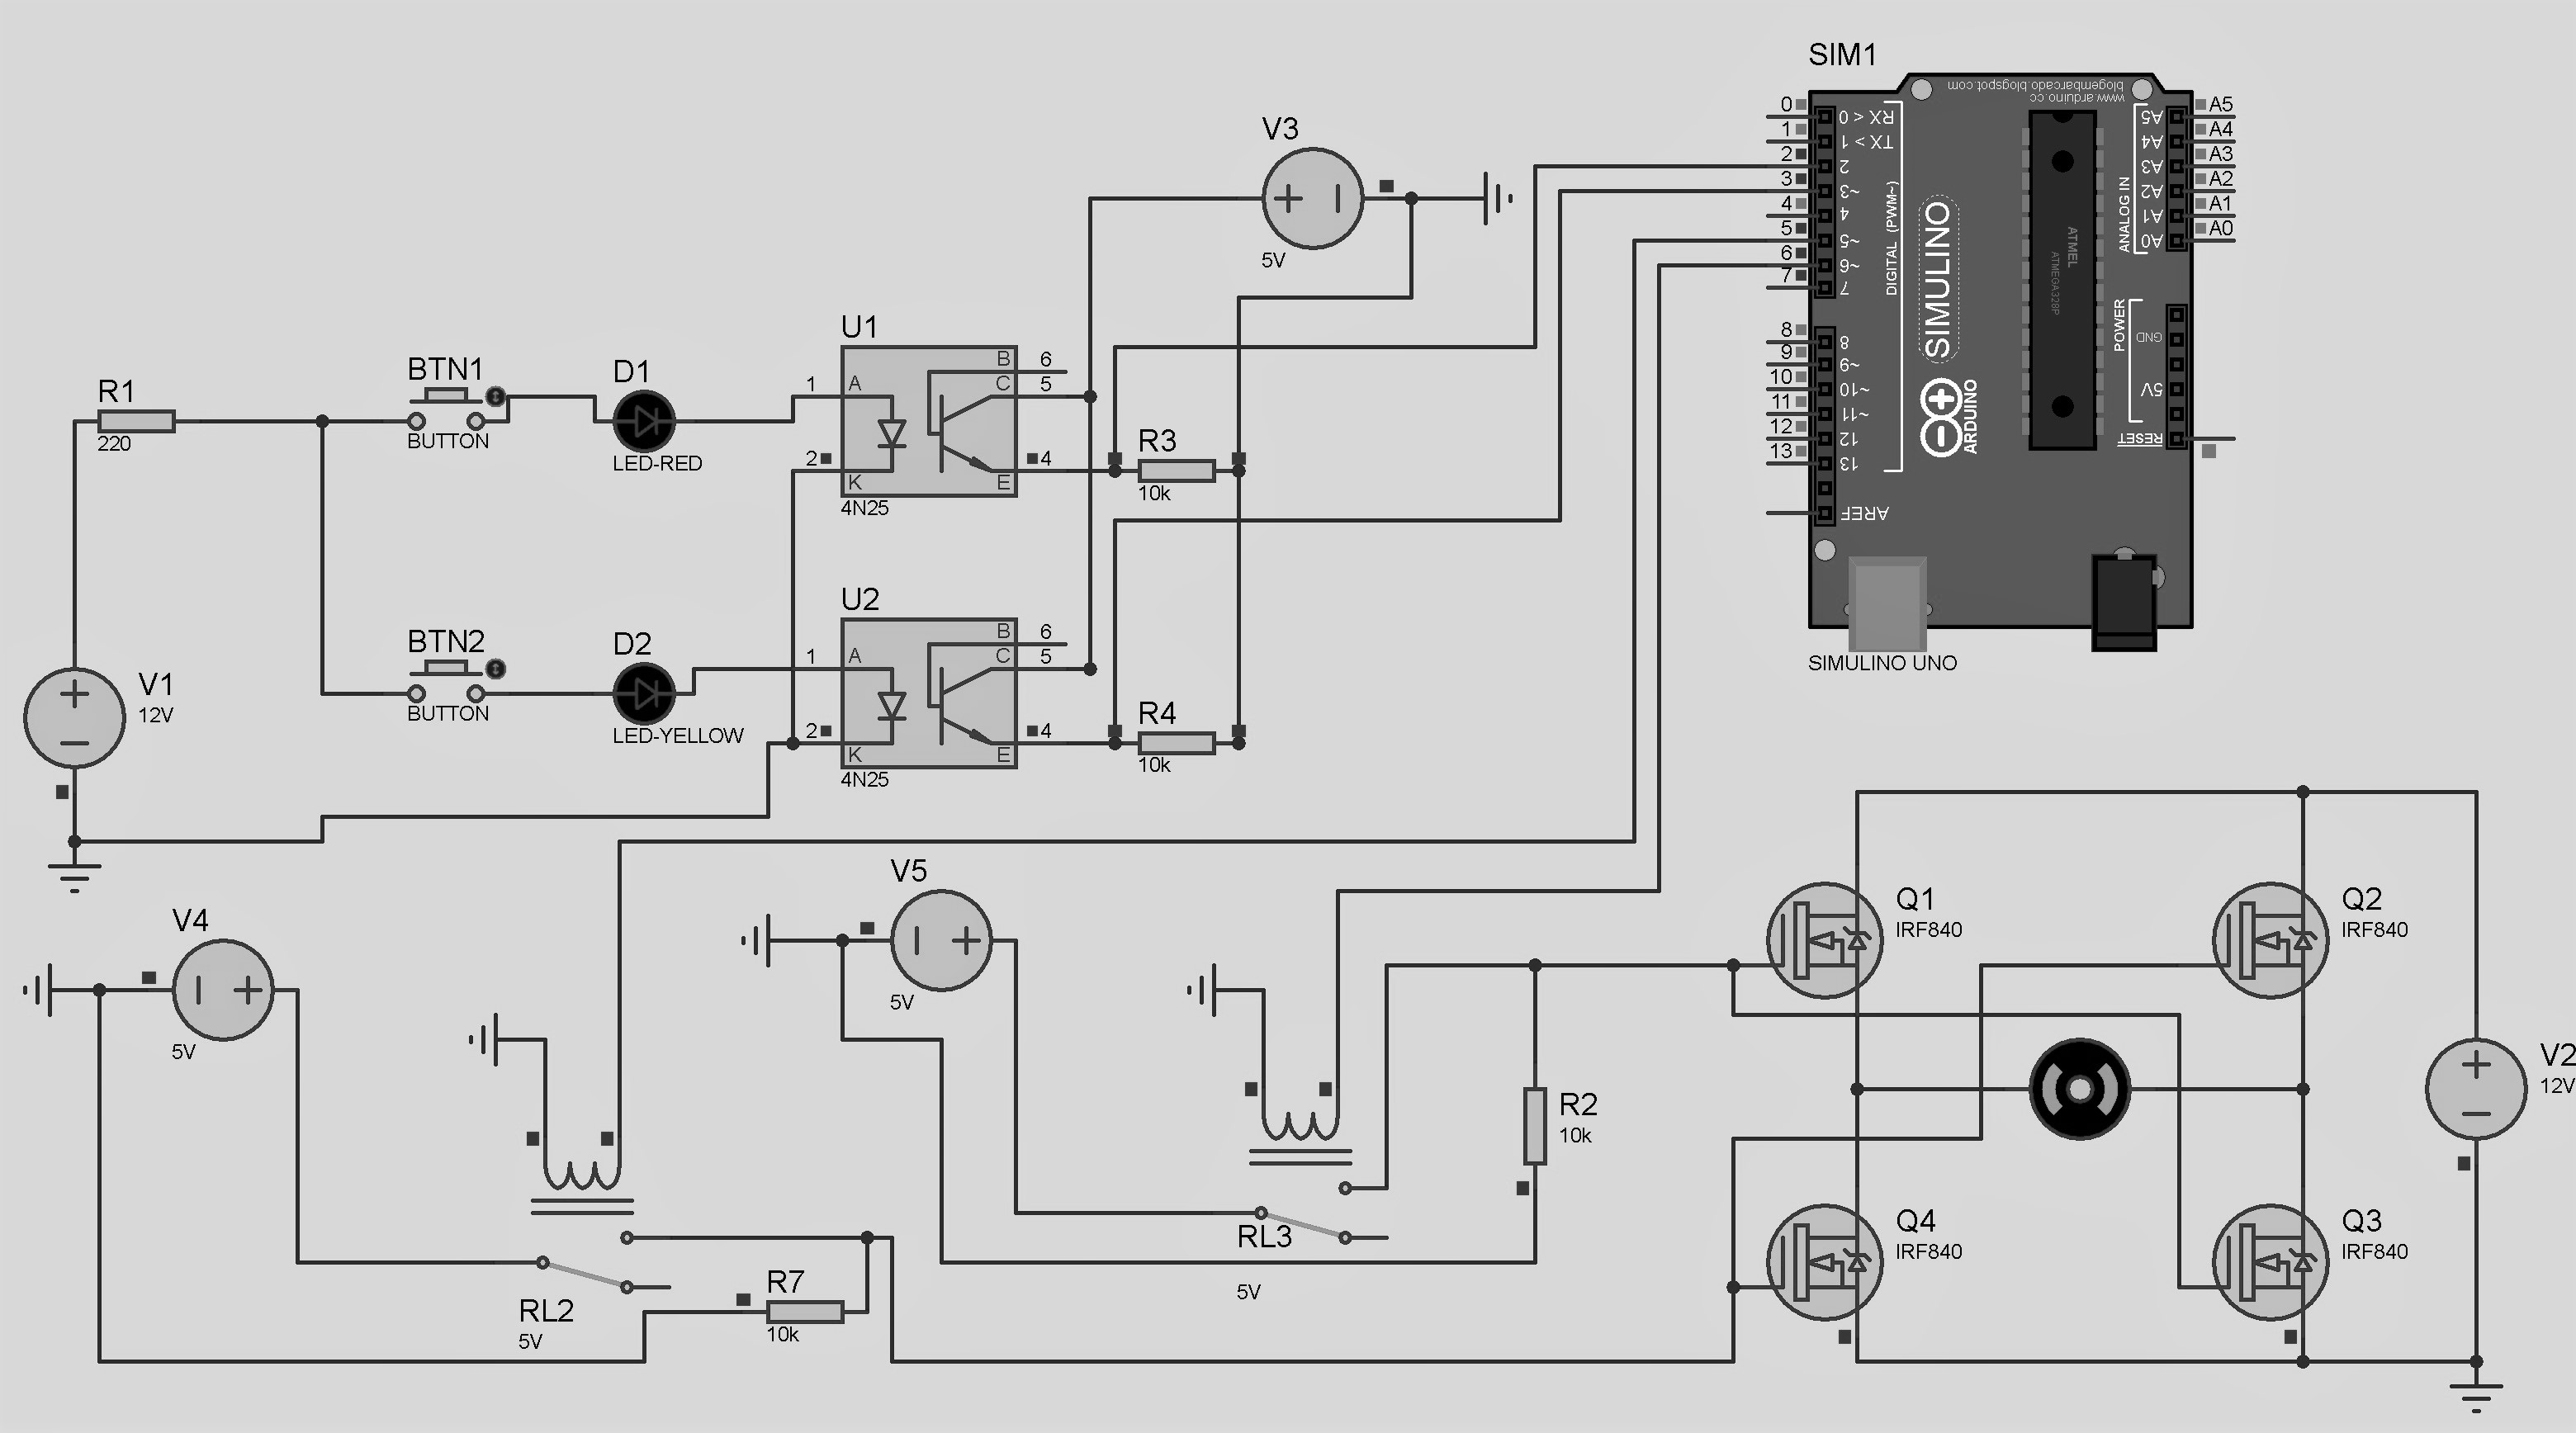
\includegraphics[scale=0.19]{imagenes/circuito.JPG}
\newpage
\begin{flushleft}
\subsection{Desarrollo de la práctica}
Antes de armar el circuito realizamos los cálculos correspondientes a las resistencias necesarias de acuerdo a la siguiente formula: \\
\end{flushleft}
\begin{center}
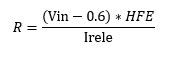
\includegraphics[scale=1]{imagenes/formula.JPG} 
\end{center}
Sustituimos valores y nos queda:
\begin{center} 
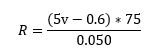
\includegraphics[scale=1]{imagenes/formula2.JPG} \\
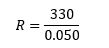
\includegraphics[scale=1]{imagenes/formula3.JPG} \\
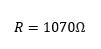
\includegraphics[scale=1]{imagenes/formulafin.JPG} \\
\end{center}
Después de tener nuestros cálculos armamos nuestro circuito y nos queda de la siguiente forma:\linebreak

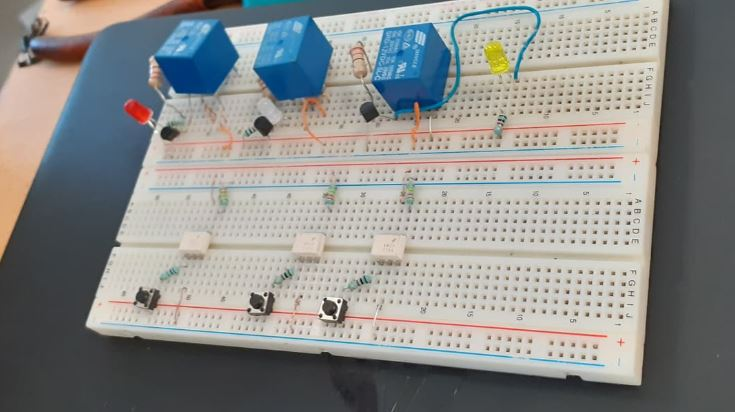
\includegraphics[scale=0.9]{imagenes/circuito1.JPG} 
\newpage
\begin{flushleft}
Al tener todo nuestro circuito conectado y nuestro arduino con el programa previamente cargado podemos darnos cuenta que el circuito hace lo que se pedía, en este caso se requeria encender un led a traves del arduino simulando el CPU de un PLC.\linebreak
\end{flushleft}
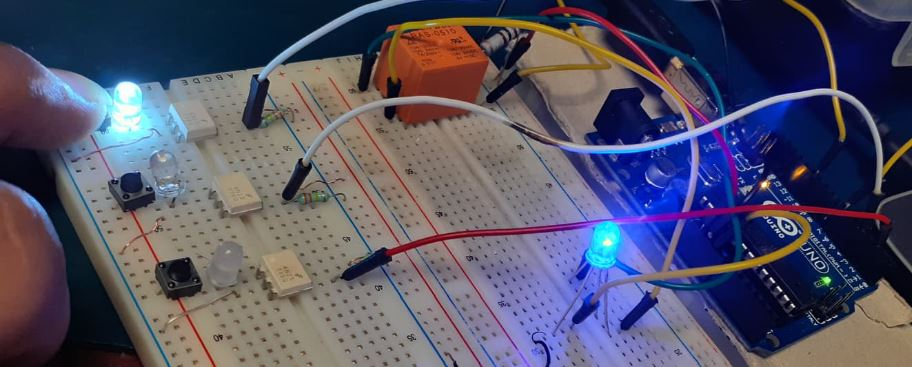
\includegraphics[scale=0.7]{imagenes/simu2.JPG}
\subsection{Funcionamiento final}
\begin{flushleft}
finalmente con el circuito como se muestra en la simulación tenemos el resultado el cual consta de 3 entradas y 3 salidas, pero lo que hace importante a estos circuitos es que con ellos podemos aislar nuestra CPU de posibles daños por problemas que ocurran fuera de nuestro PLC por ellos estos circuitos de entrada y de potencia a la salida podemos usar dispositivos mas grandes y mucho mas potentes. 
\linebreak
\linebreak
\end{flushleft}
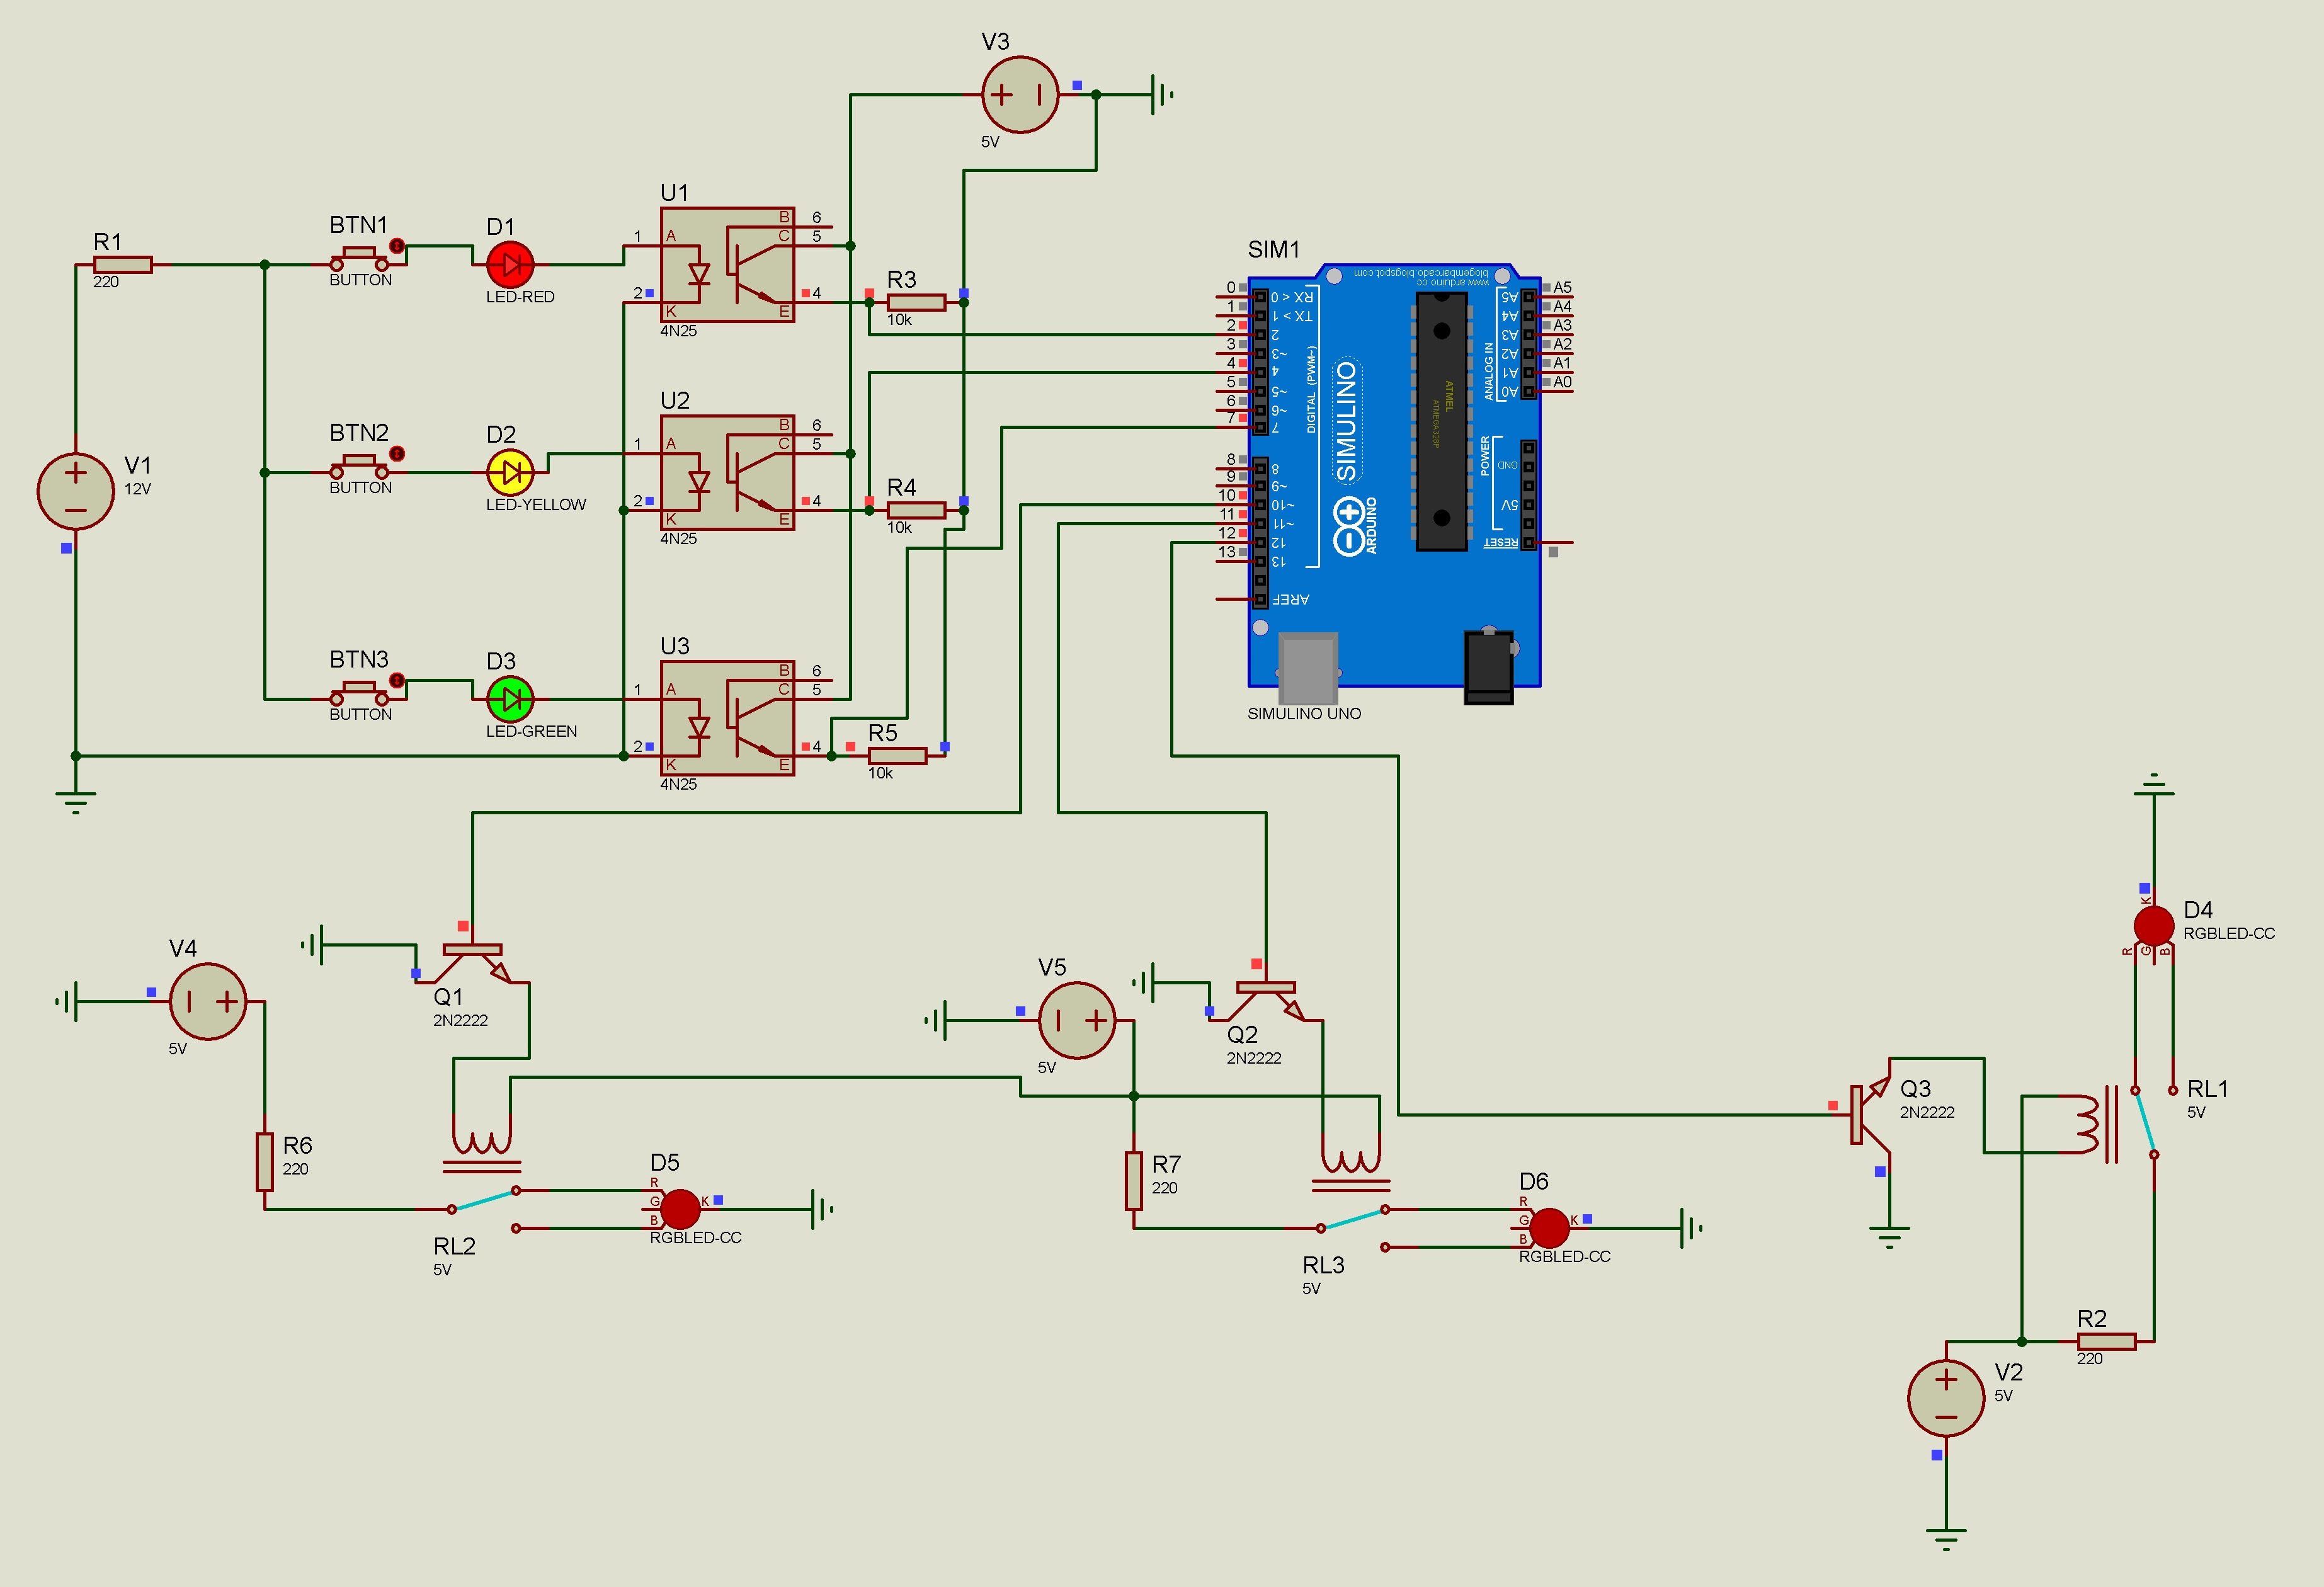
\includegraphics[scale=0.15]{imagenes/simu0.JPG}
\newpage
\subsection{Conclusiones}
\begin{flushleft}
En esta practica pudimos aprender mas sobre cono funcionan internamente los controladores lógico programables (PLC), lo que mas me pareció importante en ello es como el CPU es aislado para poder protegerse de cualquier tipo de mal funcionamiento en alguna de las terminales ya sea de entrada o de salida de esta manera el sistema es mas seguro para ser usado en todo tipo de tareas.
\end{flushleft}
\end{document}

\section{se}